\documentclass[11pt]{article}
\usepackage{graphicx, placeins}

\title{Investigate the relationship between varying the initial height of a marble rolling down
a ramp and the maximum compressed distance of a horizontal spring at the bottom
upon collision with the marble}
\date{IB Physics IA}

\begin{document}
    \maketitle
    \newpage
    \tableofcontents
    \newpage
    \section{Introduction}
    The inspiration for this experiment came from a childhood game with my brother. We used to play a game where we drop a marble down a ramp with a spring at the bottom, and when the marble hits the spring it will bounce back up the ramp, and whoever’s marble reaches the highest point wins. I have always been fascinated by this, and now I want to actually see how much the spring is compressed when the marble is dropped onto it and observe its behavior. This can then be applied to making marble machines, marble tracks, etc. when you need to determine a spring's compression to activate a latch or a different mechanism.
    \section{Research Question}    
    What is the relationship between varying initial height of a marble rolling down a ramp and
the maximum compressed distance of a horizontal spring at the bottom upon collision with
the marble?
    \section{Theory \& Background Knowledge}
    The law of conservation of energy states that the total energy of an isolated system will always be constant
\begin{equation}
    E_i=E_f \label{eqn1}
\end{equation}
Where $E_i$ is the initial energy and $E_f$ is the final energy.\\
Now consider the system of the marble and spring, its initial energy will be the gravitational potential energy when the marble is on top of the ramp.
\begin{equation}
    E_i=mgh_0 \label{eqn2}
\end{equation}
Where $m$ is the mass of the marble, $g$ is the gravitational acceleration of the Earth, and $h_0$ is the initial height of the marble.\\
The final energy at the moment when the spring is compressed the most will be the elastic potential energy of the spring and the marble
\begin{equation}
    E_f=\frac{1}{2}kx^2 \label{eqn3}
\end{equation}
Where $k$ is the spring constant, and $x$ is the maximum compression of the spring.\\
Note there is no kinetic energy here because the velocity of the marble is 0 when the spring reaches maximum compression.\\
Combining (\ref{eqn1}), (\ref{eqn2}) and (\ref{eqn3})
\begin{equation}
    mgh_0=\frac{1}{2}kx^2
\end{equation}
This equation means the gravitational potential energy lost by the marble $mgh_0$ is equal to the elastic potential energy $\frac{1}{2}kx^2$ gained by the spring when the spring is at maximum compression upon collision. \\
Isolating $x^2$ we get:
\begin{equation}
    x^2=\frac{2mg}{k}h_0
\end{equation}
    \section{Hypothesis}
    From the linearised equation $x^2=\frac{2mg}{k}\cdot h_0$ , we can plot $x^2$ against $h_0$ and obtain a linear line passing through the origin with an expected gradient of $\frac{2mg}{k}$. By comparing this against a directly calculated value of $\frac{2mg}{k}$ through direct measurement and literature value, we can determine the experimental error.
\FloatBarrier
\begin{figure}[!htb]
    \begin{center}
        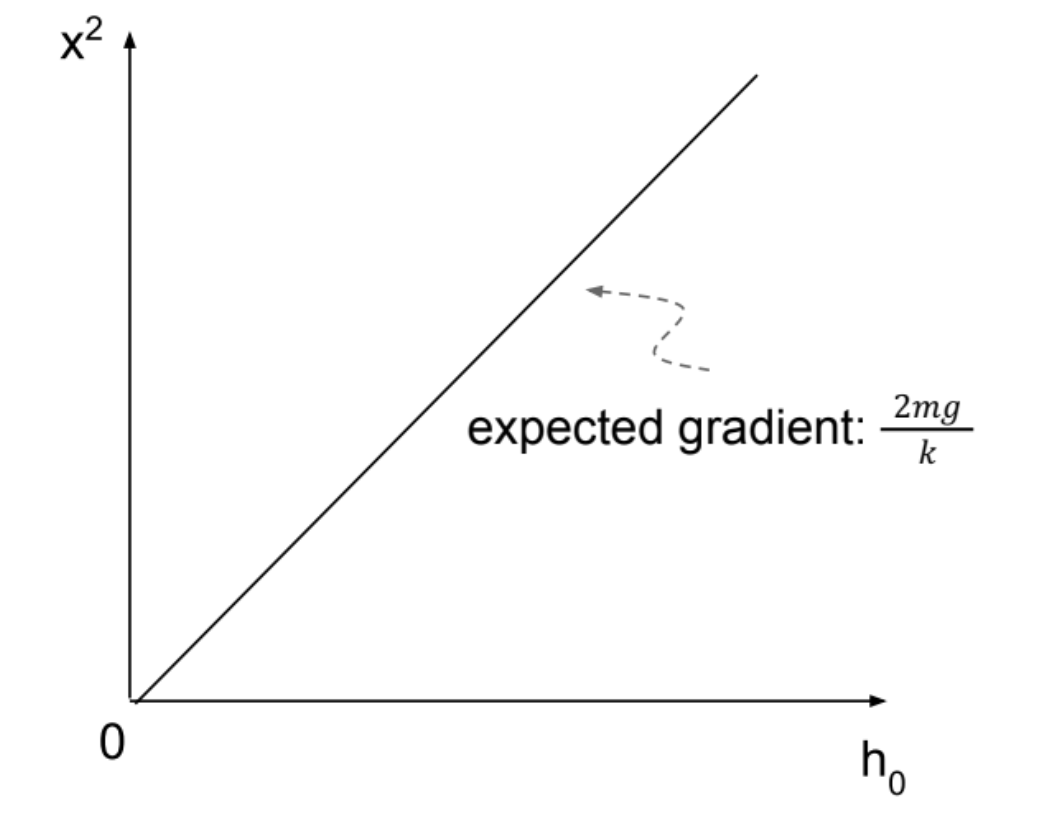
\includegraphics[width = 200px]{grad.png}
        \caption{Expected form of $x^2$ vs $h_0$ graph} \label{fig1}
    \end{center}
\end{figure}
\FloatBarrier
    \section{Variables}
    Independent variable: height of drop \\
Dependent variable: compression of spring \\ 
Controlled variables: mass of marble, spring constant, location of experiment (for constant $g$ value)
    \section{Experimental Setup}
    \FloatBarrier
\begin{figure}[!htb]
    %\begin{center}
    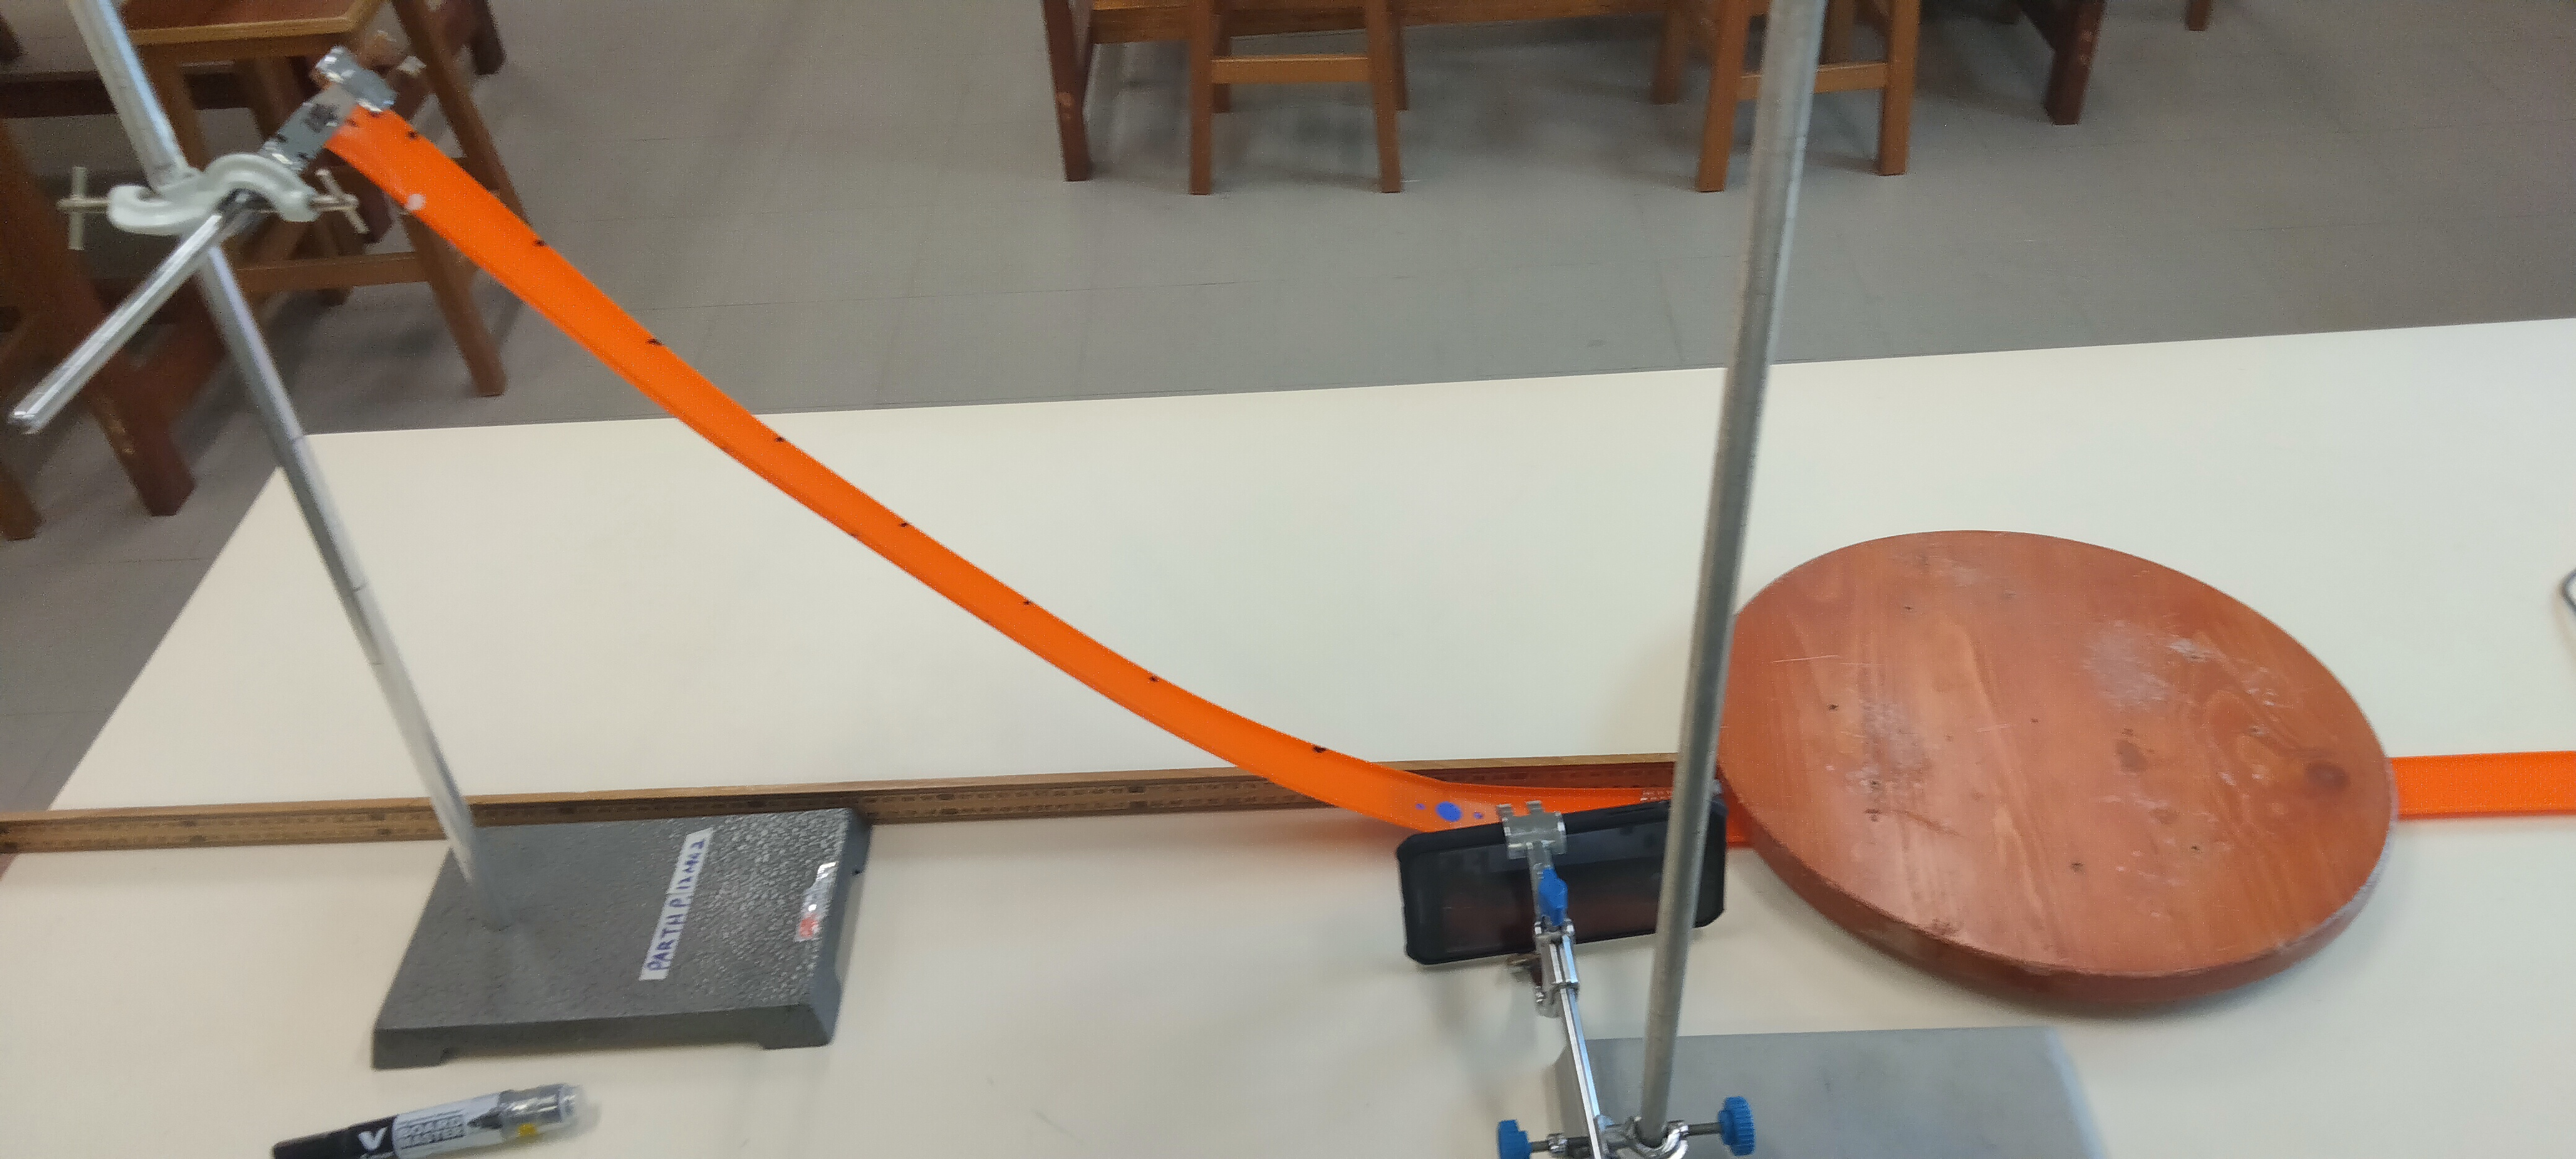
\includegraphics[width = \textwidth]{setup1.jpg}
    \caption{General set up}
\end{figure}
\begin{figure}[!htb]
    %\begin{center}
    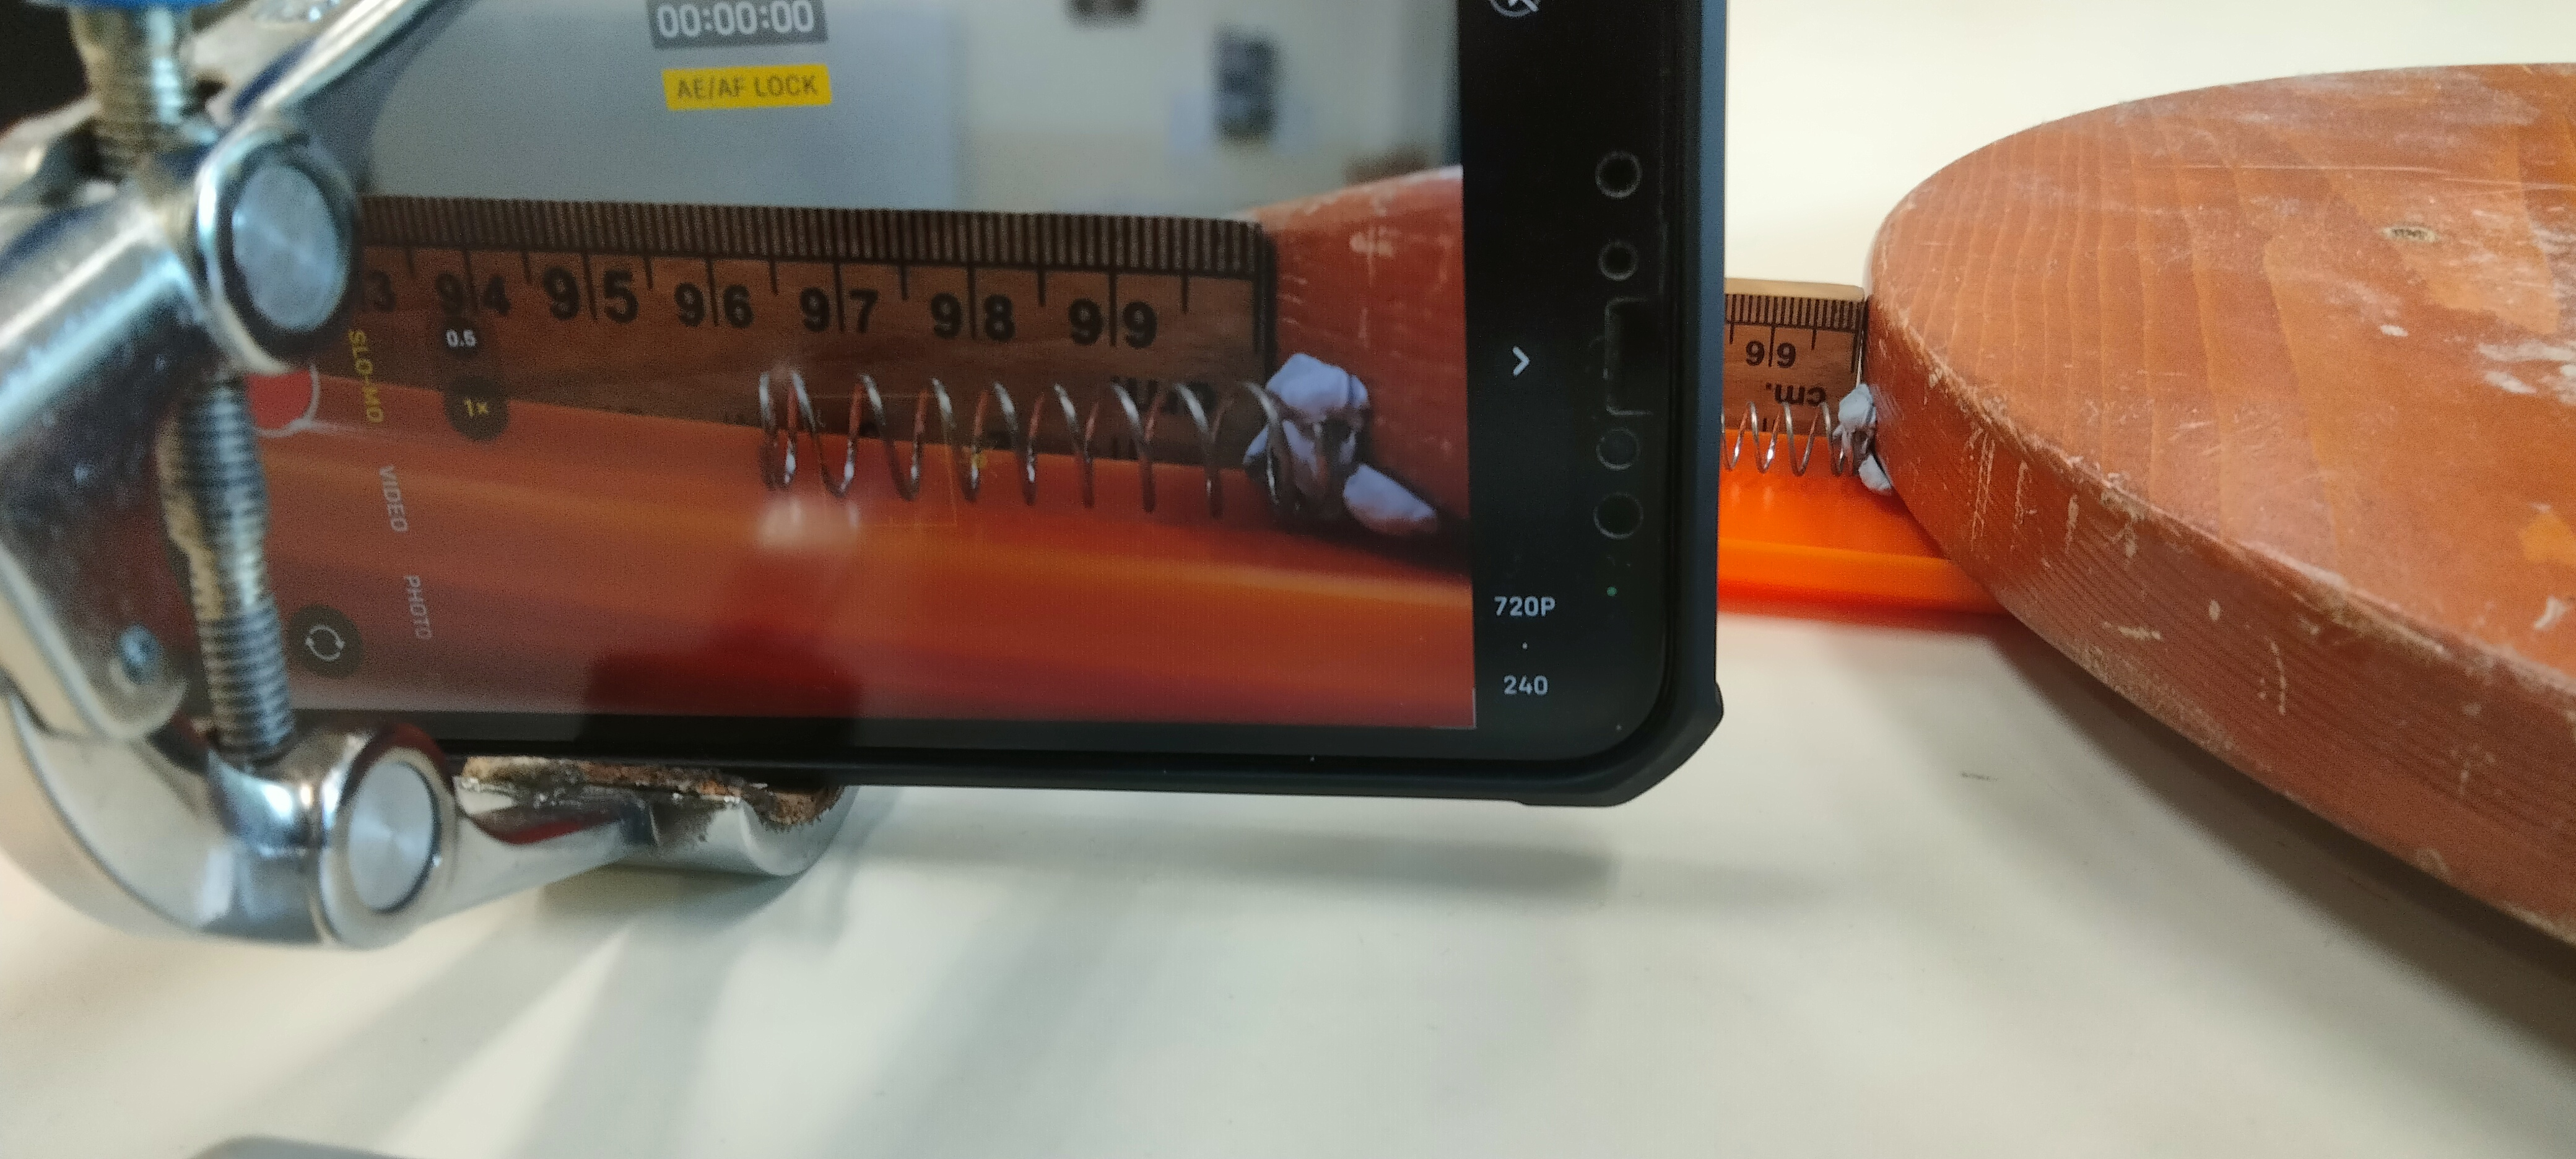
\includegraphics[width = \textwidth]{setup2.jpg}
    \caption{Set up of high speed camera \& spring}
\end{figure}
\FloatBarrier
        \subsection{Apparatus}
        \begin{itemize}
    \item 1 marble (diameter roughly 1-1.5 cm)
    \item 2 retort stand \& clamps
    \item 1 spring with known spring constant
    \item 1 long flexible track (>70cm) (can use a hot wheel track)
    \item 1 high speed camera (minimum 240 fps)
    \item 1 block of wood
\end{itemize}
        \subsection{Method}
        \begin{enumerate}
    \item Clamp 1 head of track to retort standand weigh down the other end to make a ramp for the marble as shown in Fig. \ref{fig2}. The curvature or path and shape of the ramp doesn't matter as long as there is a horizontal segment at the end, because we just need to control the drop height.
    \item Use meter rule to measure height from table of different points and make markings (40, 35, 30, 25, 20, 15, 10, 5 cm). The uncertainty of these markings will be 1mm as this is the uncertainty of the meter rule.
    \item Using Blu-tack, attach the spring to the wood block so that the spring lies on the track
    \item Set up meter rule behind the track and the spring to measure the compression
    \item Set up high speed camera in line with and focusing on the spring end 
    \item Record drop of marble from 40cm mark on ramp
    \item Repeat step 6 five more times to reduce random error
    \item Repeat steps 7 \& 8 eight more times from different markings (35, 30, 25, 20, 15, 10, 5 cm)
    \item Analyse the high speed footage frame by frame to determine and record the maximum spring compression for each drop.
\end{enumerate}
        \subsection{Risk Assessment}
        \begin{table}[!htb]
    \begin{center}
        \begin{tabular}{|l|p{5cm}|p{5cm}|} 
            \hline
            ~ & Risks & Prevention \\ 
            \hline
            \multirow{3}{4em}{Safety} & End of retort stand may be pointy and may poke eye if not careful & Wear safety glasses, handle with care \\ 
            \cline{2-3}
            & Retort stand and wood blocks can be heavy, may fall off table and onto feet & Handle with care, wear shoes in lab, make sure setup is stable in the middle of the tabletop and there's sufficient space to work.\\
            \cline{2-3}
            & Marble may bounce off spring into eye & Wear safety glasses \\
            \hline
            Environmental & None & None \\
            \hline
            Ethical & None & None  \\ 
            \hline
        \end{tabular}
        \caption{Risks \& Preventions}
    \end{center}
\end{table}
\newpage
    \section{Raw Data Table}
    \FloatBarrier
\begin{table}[!htb]
    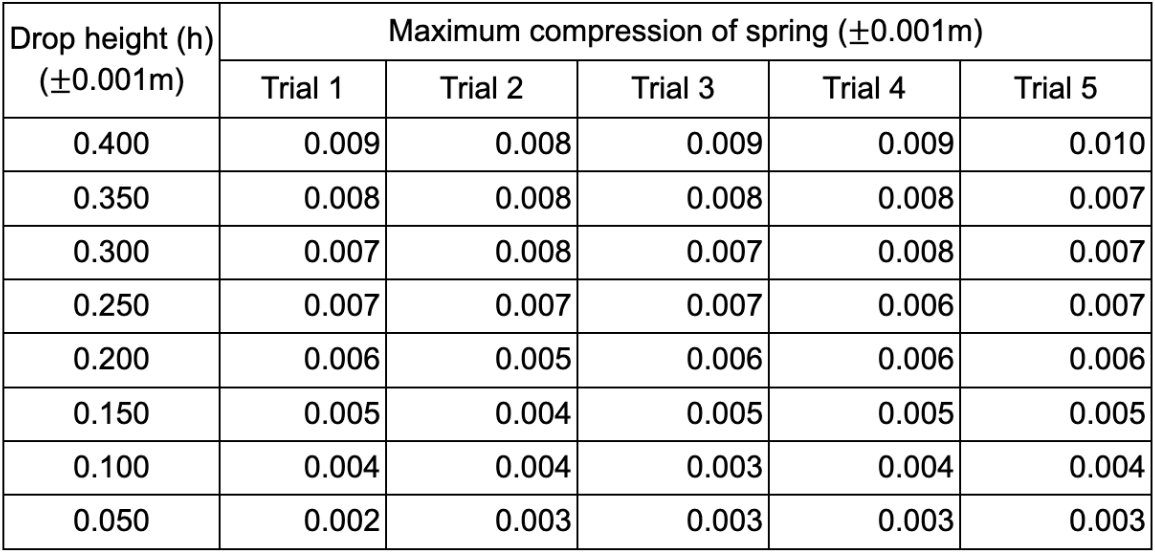
\includegraphics[width = \textwidth]{rawtbl.png}
    \caption{Table of raw data}
\end{table}
\FloatBarrier
The uncertainty of the compression is ±0.0005m (0.5mm) because the smallest scale division of the meter rule is 1mm. The uncertainty of the drop height is 0.001m (1mm) to take into account the thickness of the markings on the ramp causing small inconsistencies between drops
    \section{Processed Data Table}
    \FloatBarrier
\begin{figure}
    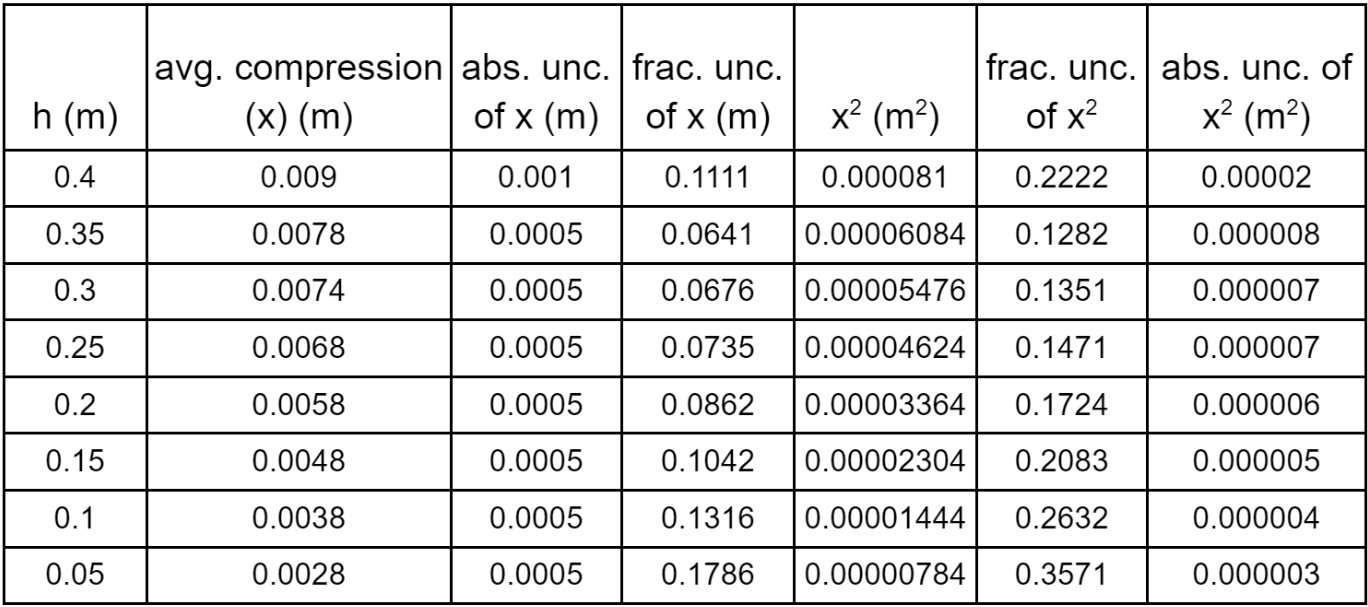
\includegraphics[width = \textwidth]{proctbl.png}
    \caption{Table of processed data}
\end{figure}
\FloatBarrier
    \section{Example Calculations}
    \begin{enumerate}
    \item $x$(average compression) = average of Trial 1 to Trial 5 values \\
    e.g. $\frac{0.009 + 0.008 + 0.009 + 0.009 + 0.010}{5} = 0.009$
    \item $\Delta$x (absolute uncertainty of $x$) = half range of Trial 1 to Trial 5 values. \\
    e.g. $\frac{0.010 - 0.008}{2} = 0.001$
    \item $\frac{\Delta x}{x}$ (fractional uncertainty of $x$) = $\Delta{x} / {x}$\\
    e.g. $\frac{0.001}{0.009} = 0.1111$
    \item $x^2$ = $x$ squared \\
    e.g. $0.009^2$ = 0.000081
    \item $\frac{\Delta x^2}{x^2}$ (fractional uncertainty of $x^2$) = $2 \cdot \frac{\Delta x}{x}$ \\
    e.g. $0.1111\cdot 2 = 0.2222$
    \item $\Delta x^2$ (absolute uncertainty of $x^2$) = $\frac{\Delta x^2}{x^2} \cdot x^2$  \\
    e.g. $0.2222 \cdot 0.000081 = 0.00002 $
\end{enumerate}
    \section{Processing \& Graphs}
    \FloatBarrier
\begin{figure}
    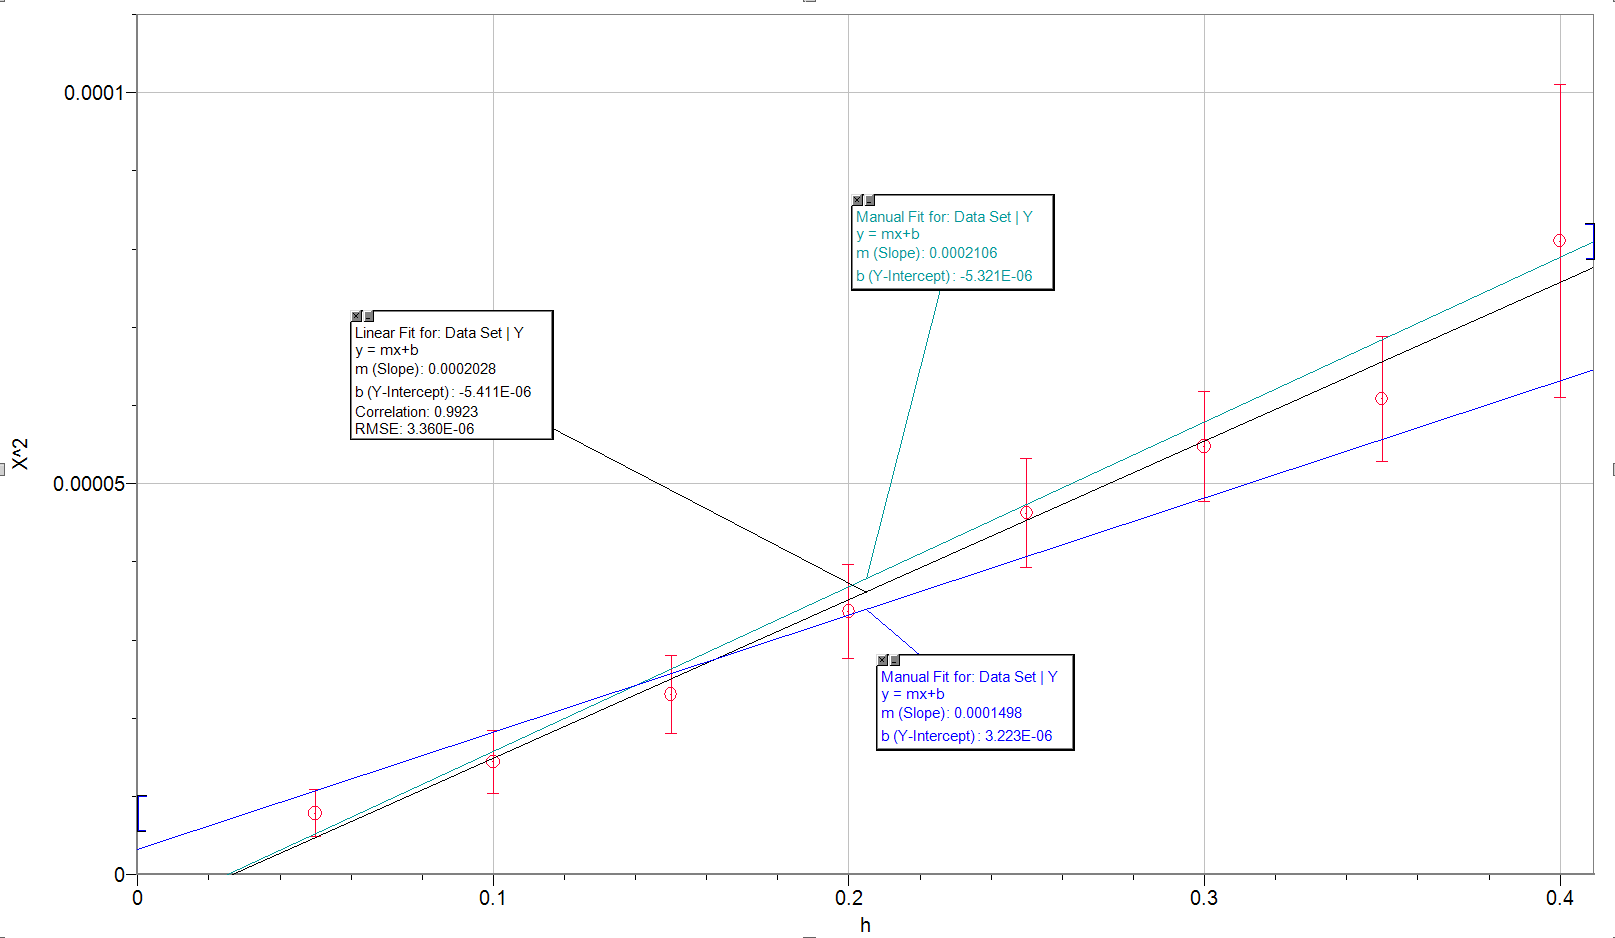
\includegraphics[width = \textwidth]{graph.png}
    \caption{Graph of $x^2$ vs $h$}
\end{figure}
\FloatBarrier
From the graph, there is a positive correlation between $x^2$ and $h$. The best fit line has an equation of $y = 0.0002028x - 0.000005411$. Compared to the directly proportional relationship as expected, there is a small systematic error. This is probably caused by the fact that the marble drop height is measured from the surface of the table, while the spring lies on the track itself, not the table surface, so there is a small difference in height. There is no significant anomaly in the data
    \section{Calculations}
    By calculating the value of g from the gradient and comparing it to the accepted literature value of g, we can determine the experimental error and use it to evaluate the accuracy of the experiment. \\
Gradient of the line of best fit is 0.0002028. Maximum gradient is 0.0002106 and minimum is 0.0001498. \\
Gradient = 2mgk \\
with m: mass of marble: 0.0065kg, and k: spring constant of the spring being used: 600N/m \\
→ g best fit = 0.0002028 * 600 / (2 * 0.0065) = 9.36 ms-2
g max = 0.0002106 * 600 / (2 * 0.0065) = 9.72 ms-2
g min = 0.0001498 * 600 / (2 * 0.0065) = 6.91 ms-2
range = (9.72 - 6.91) / 2 = 1.41
so we get the value of g is g = 9.361.04 ms-2
comparing this with accepted literature value of g = 9.81 ms-2 (International Baccalaureate Organization, 2016)
percentage experimental error = (9.81 - 9.36) / 9.81 * 100% = 4.59%

    \section{Conclusion}
    From the graph, we can see the best fit and manually fitted lines pass through all data points’ error bars. The horizontal error bars (0.001m each) are very small and cannot be seen on the graph compared to scale, so I didn’t attempt to fit the lines through them, only the vertical error bars. 
It can be observed that x2 and h are linearly correlated with proportionality constant of 0.0002028. From this, the experimental value of g can be determined to be 9.361.04 ms-2, which when compared with the accepted literature value of 9.81 ms-2, gives the percentage experimental error of 4.59\%. This experimental error is possibly due to the fact that energy is not fully conserved during the drop, and a little bit was lost as heat due to friction between the marble and the slope, but this was a small amount because both are relatively smooth surfaces. This can also be caused when the marble lightly bumps against the wall of the track when rolling down, dissipating energy. The graph does not pass through the origin due to a very small amount of systematic error. This could be due to a small zero error in my meter rule used to measure and mark out heights on the track, and also the thickness of the track. However, we can easily take these into account and minimize the systematic error to better confirm the relationship. Overall, the low values of experimental and systematic errors supports my Research Question and hypothesis, and shows that there is a linear relationship between varying initial height of a marble rolling down a ramp and the maximum compressed distance of a horizontal spring at the bottom upon collision.
    \section{Evaluation}
        \subsection{Strengths of Investigation}
        \begin{center}
    \begin{tabular}{|p{5cm}|p{5cm}|} 
        \hline
        Strength & Significance \\ 
        \hline
        Simple experiment setup & Make the experiment easily repeatable and replicable \\ 
        \hline
        Experiment carried out at the exact same geographical location & Ensuring consistency in g value. \\
        \hline
        Five trials per height, repeated with eight different heights with large range, total 40 data points & Reduce random error, increase precision of result. \\
        \hline
    \end{tabular}
\end{center}
        \subsection{Weaknesses of Investigation}
        \begin{center}
    \begin{tabular}{|p{4cm}|p{4cm}|p{4cm}|} 
        \hline
        Weakness & Significance & Improvement \\ 
        \hline
        Use of high speed camera & Low significance, however the equipment can be expensive and difficult to obtain & Find alternative ways to measure maximum spring compression \\ 
        \hline
        Visual analysis of maximum point through high speed camera footage & High significance, the limited frame rate of the camera means on some trials the moving spring end gets blurry and makes it difficult to determine the maximum compression. & Use high speed camera with higher frame rate \\
        \hline
        Friction of marble on ramp & Low significance, heat dissipated from friction of the marble on the ramp is not considered in the conservation of energy equation but the ramp and the marble are both relatively smooth so this is not a significant component & Lubricate the ramp \\
        \hline
        This is not a problem in my experiment, but a possible problem that might arise is when using weak springs, the force from the marble might cause deformation of the spring and change spring constant & High significance, this will cause the data points for higher drops to be unreliable and no longer linear & Choose spring with sufficient constant. In this case my spring has spring constant of 600N/m, which I believe is enough for my experiment \\
        \hline
    \end{tabular}
\end{center}
    \bibliographystyle{apastyle}
    \bibliography{refs.bib}
\end{document}